%!TeX encoding = UTF-8
%!TeX program = xelatex
\documentclass[notheorems, aspectratio=54, compress]{beamer}
% aspectratio: 1610, 149, 54, 43(default), 32

\usepackage{ctex}
\usepackage{latexsym}
\usepackage{amsmath,amssymb}
\usepackage{mathtools}
\usepackage{color,xcolor}
\usepackage{graphicx}
\usepackage{algorithm}
\usepackage{amsthm}
\usepackage{lmodern} % 解决 font warning
% \usepackage[UTF8]{ctex}
\usepackage{animate} % insert gif

\usepackage{lipsum} % To generate test text 
\usepackage{ulem} % 下划线,波浪线

\usepackage{listings} % display code on slides; don't forget [fragile] option after \begin{frame}

% ----------------------------------------------
% tikx
\usepackage{framed}
\usepackage{tikz}
\usepackage{pgf}
\usepackage{hyperref}
\usepackage{cite}
\usetikzlibrary{calc,trees,positioning,arrows,chains,shapes.geometric,%
    decorations.pathreplacing,decorations.pathmorphing,shapes,%
    matrix,shapes.symbols}
\pgfmathsetseed{1} % To have predictable results
% Define a background layer, in which the parchment shape is drawn
\pgfdeclarelayer{background}
\pgfsetlayers{background,main}

% define styles for the normal border and the torn border
\tikzset{
  normal border/.style={orange!30!black!10, decorate, 
     decoration={random steps, segment length=2.5cm, amplitude=.7mm}},
  torn border/.style={orange!30!black!5, decorate, 
     decoration={random steps, segment length=.5cm, amplitude=1.7mm}}}

% Macro to draw the shape behind the text, when it fits completly in the
% page
\def\parchmentframe#1{
\tikz{
  \node[inner sep=2em] (A) {#1};  % Draw the text of the node
  \begin{pgfonlayer}{background}  % Draw the shape behind
  \fill[normal border] 
        (A.south east) -- (A.south west) -- 
        (A.north west) -- (A.north east) -- cycle;
  \end{pgfonlayer}}}

% Macro to draw the shape, when the text will continue in next page
\def\parchmentframetop#1{
\tikz{
  \node[inner sep=2em] (A) {#1};    % Draw the text of the node
  \begin{pgfonlayer}{background}    
  \fill[normal border]              % Draw the ``complete shape'' behind
        (A.south east) -- (A.south west) -- 
        (A.north west) -- (A.north east) -- cycle;
  \fill[torn border]                % Add the torn lower border
        ($(A.south east)-(0,.2)$) -- ($(A.south west)-(0,.2)$) -- 
        ($(A.south west)+(0,.2)$) -- ($(A.south east)+(0,.2)$) -- cycle;
  \end{pgfonlayer}}}

% Macro to draw the shape, when the text continues from previous page
\def\parchmentframebottom#1{
\tikz{
  \node[inner sep=2em] (A) {#1};   % Draw the text of the node
  \begin{pgfonlayer}{background}   
  \fill[normal border]             % Draw the ``complete shape'' behind
        (A.south east) -- (A.south west) -- 
        (A.north west) -- (A.north east) -- cycle;
  \fill[torn border]               % Add the torn upper border
        ($(A.north east)-(0,.2)$) -- ($(A.north west)-(0,.2)$) -- 
        ($(A.north west)+(0,.2)$) -- ($(A.north east)+(0,.2)$) -- cycle;
  \end{pgfonlayer}}}

% Macro to draw the shape, when both the text continues from previous page
% and it will continue in next page
\def\parchmentframemiddle#1{
\tikz{
  \node[inner sep=2em] (A) {#1};   % Draw the text of the node
  \begin{pgfonlayer}{background}   
  \fill[normal border]             % Draw the ``complete shape'' behind
        (A.south east) -- (A.south west) -- 
        (A.north west) -- (A.north east) -- cycle;
  \fill[torn border]               % Add the torn lower border
        ($(A.south east)-(0,.2)$) -- ($(A.south west)-(0,.2)$) -- 
        ($(A.south west)+(0,.2)$) -- ($(A.south east)+(0,.2)$) -- cycle;
  \fill[torn border]               % Add the torn upper border
        ($(A.north east)-(0,.2)$) -- ($(A.north west)-(0,.2)$) -- 
        ($(A.north west)+(0,.2)$) -- ($(A.north east)+(0,.2)$) -- cycle;
  \end{pgfonlayer}}}

% Define the environment which puts the frame
% In this case, the environment also accepts an argument with an optional
% title (which defaults to ``Example'', which is typeset in a box overlaid
% on the top border
\newenvironment{parchment}[1][Example]{%
  \def\FrameCommand{\parchmentframe}%
  \def\FirstFrameCommand{\parchmentframetop}%
  \def\LastFrameCommand{\parchmentframebottom}%
  \def\MidFrameCommand{\parchmentframemiddle}%
  \vskip\baselineskip
  \MakeFramed {\FrameRestore}
  \noindent\tikz\node[inner sep=1ex, draw=black!20,fill=white, 
          anchor=west, overlay] at (0em, 2em) {\sffamily#1};\par}%
{\endMakeFramed}

% ----------------------------------------------

\mode<presentation>{
    \usetheme{CambridgeUS}
    % Boadilla CambridgeUS
    % default Antibes Berlin Copenhagen
    % Madrid Montpelier Ilmenau Malmoe
    % Berkeley Singapore Warsaw
    \usecolortheme{dolphin}
    % beetle, beaver, orchid, whale, dolphin
    \useoutertheme{miniframes}
    % infolines miniframes shadow sidebar smoothbars smoothtree split tree
    \useinnertheme{circles}
    % circles, rectanges, rounded, inmargin
}
% 设置 block 颜色
\setbeamercolor{block title}{bg=red!30,fg=white}

\newcommand{\reditem}[1]{\setbeamercolor{item}{fg=red}\item #1}

\setbeamertemplate{bibliography item}[text]

% 缩放公式大小
\newcommand*{\Scale}[2][4]{\scalebox{#1}{\ensuremath{#2}}}

% 解决 font warning
\renewcommand\textbullet{\ensuremath{\bullet}}

% ---------------------------------------------------------------------
% flow chart
\tikzset{
    >=stealth',
    punktchain/.style={
        rectangle, 
        rounded corners, 
        % fill=black!10,
        draw=white, very thick,
        text width=6em,
        minimum height=2em, 
        text centered, 
        on chain
    },
    largepunktchain/.style={
        rectangle,
        rounded corners,
        draw=white, very thick,
        text width=10em,
        minimum height=2em,
        on chain
    },
    line/.style={draw, thick, <-},
    element/.style={
        tape,
        top color=white,
        bottom color=blue!50!black!60!,
        minimum width=6em,
        draw=blue!40!black!90, very thick,
        text width=6em, 
        minimum height=2em, 
        text centered, 
        on chain
    },
    every join/.style={->, thick,shorten >=1pt},
    decoration={brace},
    tuborg/.style={decorate},
    tubnode/.style={midway, right=2pt},
    font={\fontsize{10pt}{12}\selectfont},
}
% ---------------------------------------------------------------------

% code setting
\lstset{
    language=C++,
    basicstyle=\ttfamily\footnotesize,
    keywordstyle=\color{red},
    breaklines=true,
    xleftmargin=2em,
    numbers=left,
    numberstyle=\color[RGB]{222,155,81},
    frame=shadowbox,
    tabsize=4,
    breakatwhitespace=false,
    showspaces=false,               
    showstringspaces=false,
    showtabs=false,
    morekeywords={Str, Num, List},
}

% \lstset{
%     basicstyle=\ttfamily\small,
%     keywordstyle=\bfseries\color{deepblue},
%     emphstyle=\ttfamily\color{deepred},    % Custom highlighting style
%     stringstyle=\color{deepgreen},
%     numbers=left,
%     numberstyle=\small\color{halfgray},
%     rulesepcolor=\color{red!20!green!20!blue!20},
%     frame=shadowbox,
% }

% ---------------------------------------------------------------------

%% preamble
\title[毕业设计开题报告]{基于开源情报的某领域知识图谱构建}
\subtitle{医疗领域中文命名实体抽取}
\author{答辩人:汪洪钧\quad 指导老师:何亮}
\institute[]{清华大学电子工程系}
\date{\today}

% -------------------------------------------------------------

\begin{document}

%% title frame
\begin{frame}
    \titlepage
\end{frame}

\begin{frame}{目录}
  \tableofcontents[sectionstyle=show,subsectionstyle=show,subsubsectionstyle=show/shaded/hide]
\end{frame}

\section{课题背景}
%% normal frame


\subsection{命名实体识别}

\begin{frame}{命名实体识别方法}
  \begin{itemize}%[<+-| alert@+>]
    \item 命名实体识别是信息抽取领域中的一项重要任务,也是许多下游智能应用
    的重要先决条件,例如决策系统和知识图谱的构造。
    \item 常见的命名实体识别任务:序列标注
    \item 命名实体识别方法:LSTM-CRF, BERT-LSTM-CRF等
    \begin{itemize}
      \item LSTM-CRF\cite{lample2016neural}通过双向LSTM建模上下文关系,通过条件随机场建模标签之间的关系
      \item BERT\cite{devlin2018bert}通过巨量语料库预训练的语言模型,可以针对各种下游任务进行微调,也可将输出接其他层进行训练
    \end{itemize}
  \end{itemize}
\end{frame}


\begin{frame}{LSTM-CRF}
  \begin{itemize}
    \item 使用Bi-LSTM学习上下文知识
    \item 使用char-embedding结合world-embedding作为Bi-LSTM的输入
    \item 使用CRF层处理Bi-LSTM的输出,得到结果
  \end{itemize}
  \begin{figure}
    \centering
    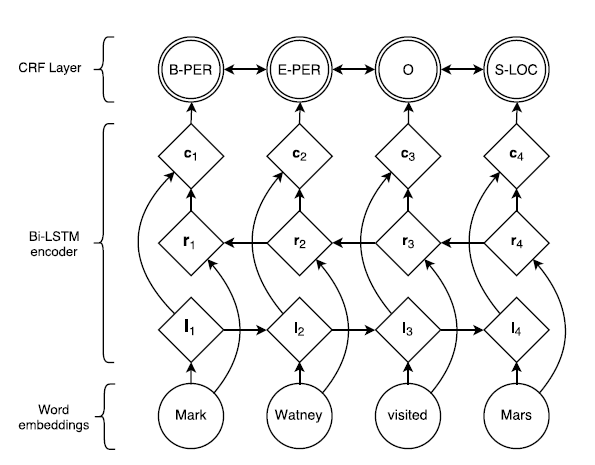
\includegraphics[width=0.8\linewidth,height=0.6\textheight,keepaspectratio]{LSTM-CRF Model}
  \end{figure}
\end{frame}

\begin{frame}{TENER}
	\begin{itemize}
		\item Transformer在NER任务上表现不佳:缺少方向信息
		\item TENER\cite{yan2019tener}使用基于相对位置(有正负)的Attention机制
	\end{itemize}
	\begin{figure}
		\centering
		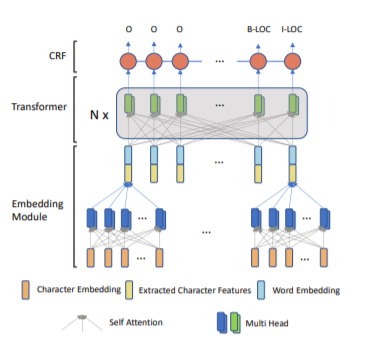
\includegraphics[width=0.8\linewidth,height=0.6\textheight,keepaspectratio]{TENER Model}
	\end{figure}
\end{frame}

\begin{frame}{BERT}
	\begin{itemize}
		\item 巨型的模型(Transformer 24 layers, 1024 dim, 16heads)与巨量的语料
		\item 训练任务一:随机掩蔽序列中的tokens,进行预测
		\item 训练任务二:输入两个句子进行是否为连续句子的判断
		\item 在多个下游任务中,包括命名实体识别取得优秀成果
	\end{itemize}
	\begin{figure}
		\centering
		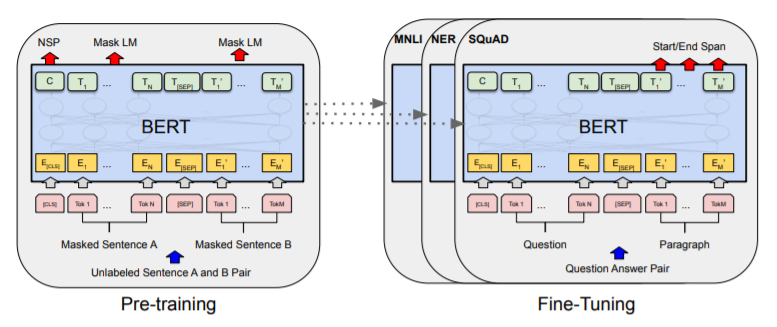
\includegraphics[width=0.8\linewidth,height=0.5\textheight,keepaspectratio]{BERT Model}
	\end{figure}
\end{frame}

\begin{frame}{BERT}
	\begin{figure}
		\centering
		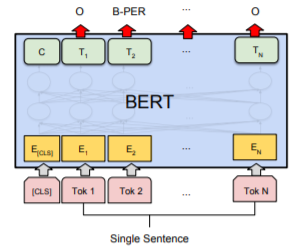
\includegraphics[width=0.8\linewidth,height=0.6\textheight,keepaspectratio]{BERT Model For NER}
	\end{figure}
\end{frame}


\section{课题内容}

\begin{frame}{课题内容}

  \begin{enumerate}
    \item 医疗领域中文命名实体识别
    \item 数据集
    \item 系统实现
  \end{enumerate}
\end{frame}

\subsection{医疗领域中文命名实体识别}

\begin{frame}{中文命名实体识别的难点}
	\begin{itemize}
		\item 中文命名实体识别的难点在于"词"的划分
		\begin{itemize}
			\item 中文序列的独特性在于其输入的单位是"字",难以实现字词结合
			\item 例如:王小美今天坐高铁来到北京南站。
			\item 经过中间步骤"分词"的效果不如仅仅以"字"为单位输入进行LSTM-CRF 	
		\end{itemize}
		\item Lattice LSTM\cite{zhang2018chinese}是词信息引入的结构的开山之作
	\end{itemize}
\end{frame}

\begin{frame}{Lattice LSTM}
	\begin{itemize}
		\item 在计算第k个单元时,除了常规LSTM的输入外,还考虑以位置k结尾的词的信息
		\item 同样地,使用Bi-LSTM和CRF
		\item 缺点:无法并行计算,难以移植到其他结构
	\end{itemize}
	\begin{figure}
		\centering
		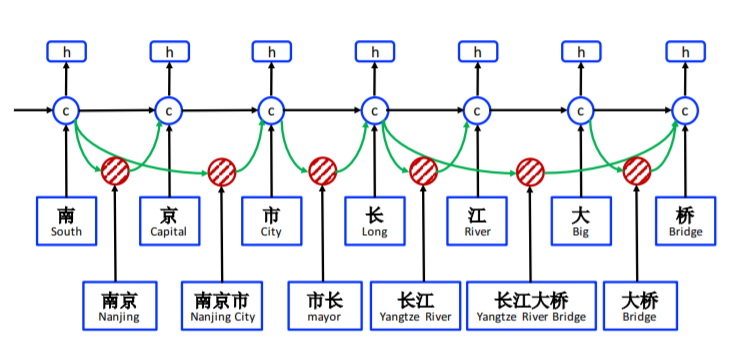
\includegraphics[width=0.8\linewidth,height=0.5\textheight,keepaspectratio]{Lattice LSTM structure}
	\end{figure}
\end{frame}

\begin{frame}{FLAT}
	\begin{itemize}
		\item FLAT\cite{li2020flat}的想法来自于Lattice和TENER等
		\item 将字和词都作为Transformer的输入,同时将它们的首尾(相对)位置也作为输入,进行基于相对位置的Attention
		\item 仅使用一层encoder
	\end{itemize}
	\begin{figure}
		\centering
		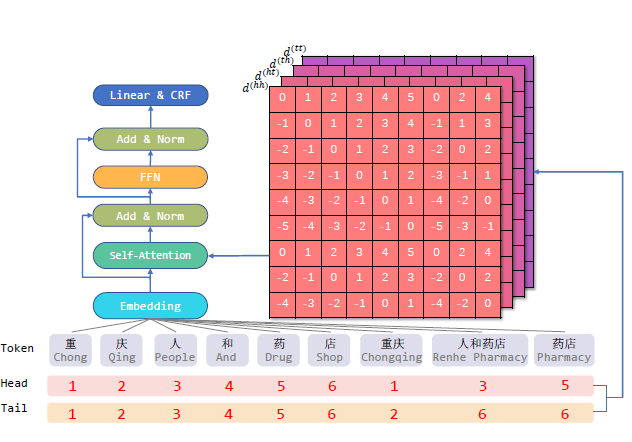
\includegraphics[width=0.8\linewidth,height=0.6\textheight,keepaspectratio]{FLAT Model}
	\end{figure}
\end{frame}

\begin{frame}{Soft-Lexicon}
	\begin{itemize}
		\item Soft-Lexicon\cite{peng2019simplify}同样是词信息的嵌入,使用的是词语的分类嵌入拼接
	\end{itemize}
	\begin{figure}
		\centering
		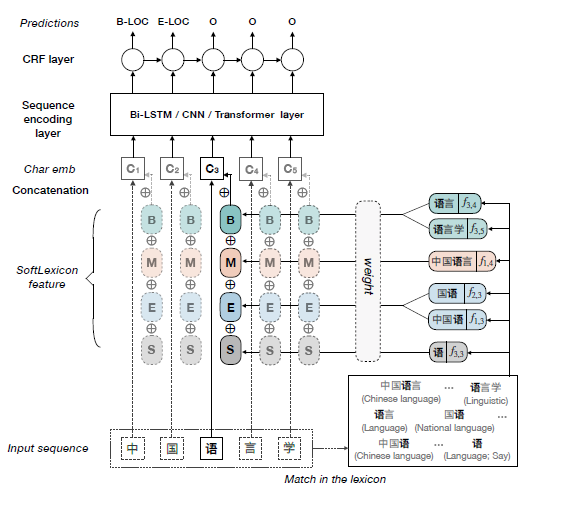
\includegraphics[width=0.8\linewidth,height=0.6\textheight,keepaspectratio]{Soft Lexicon Model}
	\end{figure}
\end{frame}

\begin{frame}{针对中文医疗领域}
  \begin{itemize}
  	\item 将尽量综合以上各个结构的优点进行系统融合
    \item 小领域的实体抽取难点在于语料的缺乏
    \begin{itemize}
      \item 将考虑实体词典(Gazetteers,含实体类型标签)强化语料
    \end{itemize}
    \item 会考虑采用一些新的结构
    \begin{itemize}
    	\item 更注重推理和全局信息的图结构
    	\item 使用新的预训练语言模型,如LUKE\cite{yamada2020luke},XLNet\cite{yang2019xlnet}
    \end{itemize}
  \end{itemize}
\end{frame}

\subsection{数据集}

\begin{frame}{中文数据集}
  \begin{itemize}
  	\item 常见的中文数据集有以下四个
    \begin{figure}
    	\centering
    	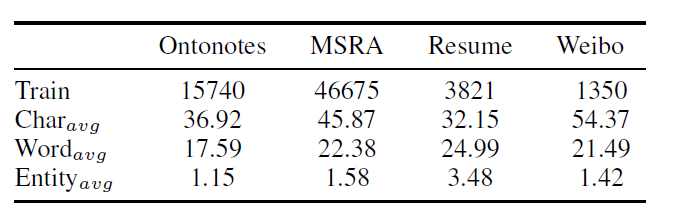
\includegraphics[width=0.8\linewidth,height=0.6\textheight,keepaspectratio]{dataset}
    \end{figure}
	\item 词信息来自Lattice-LSTM\cite{zhang2018chinese}提供
  \end{itemize}
\end{frame}

\begin{frame}{医疗领域数据集}
	\begin{itemize}
		\item 医疗领域数据集
		\begin{itemize}
			\item 具体的评测任务提供(如:CHIP2020)
			\item CCLUE:中文临床自然语言处理算法评估基准
		\end{itemize}
		\item 实体词典可以来自该领域相关的平台(比如医疗领域有医渡云)
		\item THUOCL提供医学类词信息
	\end{itemize}
\end{frame}

\subsection{系统实现}

\begin{frame}{系统实现}
  \begin{itemize}
    \item 拟定采用实体词典强化实体识别,结构化信息强化实体分类的多任务结构
    \begin{figure}
    	\centering
    	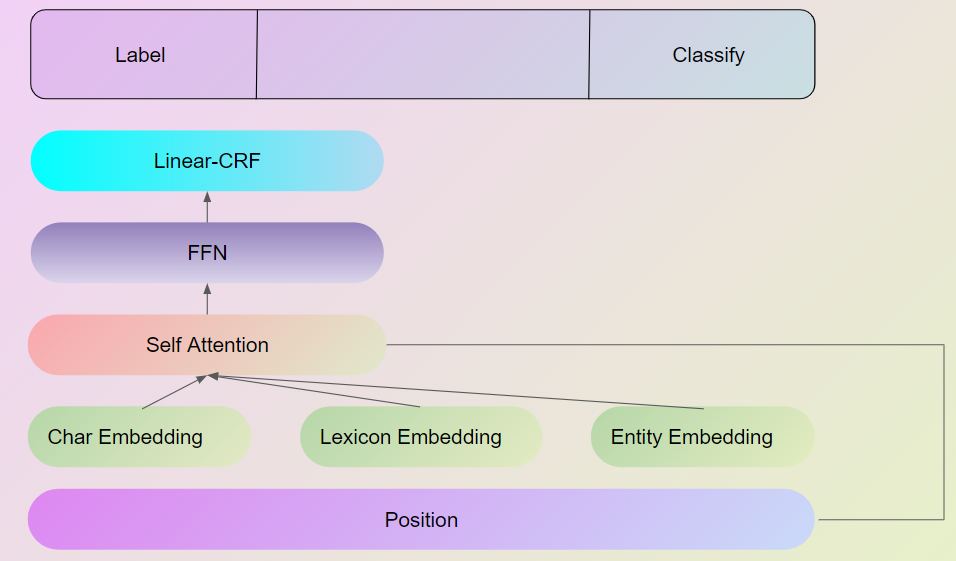
\includegraphics[width=0.8\linewidth,height=0.6\textheight,keepaspectratio]{系统框架}
    \end{figure}
    \item 拟定采用Lattice-LSTM\cite{zhang2018chinese}作为baseline
  \end{itemize}
\end{frame}
   

\section{计划进度}

\begin{frame}{计划进度}
  \begin{itemize}
    \item 2020.10-2021.12:文献调研
    \item 2021.01-2021.03:在数据集上跑通Baseline,以及其他有较好表现的系统,然后搭建自行设计的系统框架,运行系统
    \item 2021.04-2021.05:验证结果
  \end{itemize}
\end{frame}

\section{参考文献}

\begin{frame}[allowframebreaks]{参考文献}
  \tiny\bibliographystyle{ieeetr}
  \bibliography{ref}
\end{frame}

\begin{frame}
  \begin{center}
    \Huge 谢谢!
  \end{center}
\end{frame}

\end{document}